
\documentclass{beamer}
\usetheme{Warsaw}

\usepackage[spanish]{babel}
\usepackage{graphicx}

\title{Las cuentas del Gran Capitán}
\author{Perico de los Palotes}
\institute{Reino de Castilla y León}
\date{14 de diciembre de 2020}

\begin{document}

\begin{frame}
\titlepage
\end{frame}

\begin{frame}
\frametitle{Guión}
\tableofcontents
\end{frame}

\section{Orden del día}
\begin{frame}
\frametitle{Orden del día}

\begin{itemize}
\item Objetivos
\item Antecedentes
\item Descripción general
\item Conclusiones
\end{itemize}

\end{frame}

\begin{frame}
\frametitle{¡Fuera del orden del día!}

\begin{itemize}
\item Picos, palas y azadones, cien millones de ducados
\pause
\item Frailes, monjas y pobres, ciento cincuenta mil ducados
\pause
\item Guantes perfumados, cien mil ducados
\pause
\item Reponer y arreglar las campanas, ciento sesenta mil ducados
\pause
\item Pequeñeces del rey, cien millones de ducados 
\end{itemize}

\end{frame}


\section{Antecedentes}

\begin{frame}
\frametitle{Objetivos clave y  factores de éxito}

\begin{itemize}
\item Campaña de Nápoles
\begin{itemize}
\item Conquistar el reino de Nápoles
\item Ganar acceso al resto de Italia
\end{itemize}
\end{itemize}


\begin{block}{Visión compartida}
\begin{itemize}
\item La victoria ha sido total
\item Los  recursos concedidos han sido escasos
\end{itemize}
\end{block}

\end{frame}

\section{Descripción general}

\begin{frame}
\frametitle{Descripción general}

\begin{figure}
\centering
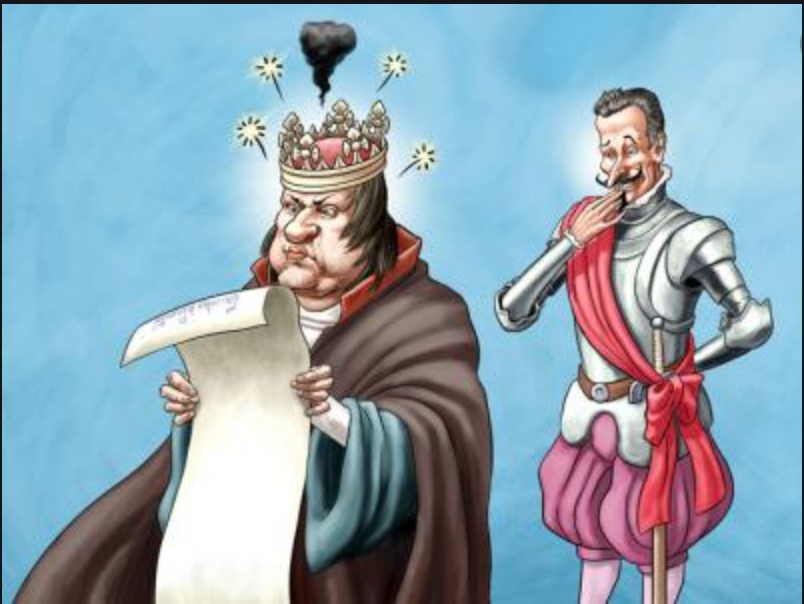
\includegraphics[width=0.40\textwidth]{cuentas}
\end{figure}

\begin{table}[]
\centering
\begin{tabular}{|l|r|r|}
\hline
Concepto          & Coste     & Coste acumulado \\ \hline
Picos, \ldots     & 100.000 K & 100.000 K \\ \hline
Frailes, \ldots   & 150 K     & 100.150 K \\ \hline
Guantes \dots     & 100 K     & 100.250 K \\ \hline
Campanas \ldots   & 160 K     & 100.410 K \\ \hline
Pequeñeces \ldots & 100.000 K & 200.410 K \\ \hline
\end{tabular}
\end{table}

\end{frame}

\section{Conclusiones}

\begin{frame}
\frametitle{Conclusiones}

\begin{columns}
% INTRODUCIMOS LA PRIMERA COLUMNA
\begin{column}{0.4\textwidth}
\begin{itemize}
\item Hemos ganado la guerra
\item Sin apenas tropas
\item Con un presupuesto reducido
\end{itemize}
\end{column}
% INTRODUCIMOS LA SEGUNDA COLUMNA
\begin{column}{0.6\textwidth}
\begin{itemize}
\item Los soldados han mostrado arrojo y generosidad
\item Han regalado un reino a España
\item No se merecen estas pequeñeces
\end{itemize}
\end{column}
\end{columns}

\end{frame}


\end{document}